\section{Simulation Results}
\label{sec:simulation_results}

In this section, we present results of an experiment in which the \emph{LinDist3Flow} equations were incorporated into an OPF with the objective of regulating system voltage magnitudes to within acceptable limits, and minimize the voltage phasor difference between a selected node and a target phasor (we refer to this as voltage phasor tracking). The OPF decision variables were DER real and reactive power injections at select nodes, which were capacity constrained (i.e. four-quadrant resources).

Prior to introducing our OPF problem, we first wish to include a brief note regarding the formulation of the voltage phasor tracking problem as an SDP.  In an effort to compare the result of our approach with an optimal effort (i.e. solving an OPF that uses the exact power flow equations), we investigated extending the works of \cite{dall2012optimization}-\cite{dall2013distributed}. Our first approach was to formulate an OPF tracking problem using the L1 norm in the objective function, however we could not obtain a tight relaxation (a rank 1 solution) for even the simplest of cases. Following this, we augmented the OPF presented in \cite{dall2013distributed} by adding equality constraints to prescribe voltage magnitude(s) and phase angle(s) at one or more nodes. Not all choices of reference voltage phasor led to a rank 1 solution however, and we would often need to repeatedly guess to find a suitable reference. Our extension of this work and derivation of constrains can be found in the appendix.
% Following the addition of these constraints, we were unable to obtain a tight relaxation (a rank 1 solution) for even the simplest of problems.

%In this modified OPF, voltage magnitudes and phase angles are specified using equality constraints (please see Appendix for derivation). While we were successful in finding feasible operating states (obtaining a rank 1 solution to the SDP), we were just as often unsuccessful (a solution of rank greater than 1 was obtained). We were also unsuccessful in eliminating the added equality constraints by transforming the OPF into a tracking problem, as we were unable to obtain a rank 1 solution for even the simplest of problems.

Our experiment was conducted on a modified version of the IEEE 37 node distribution feeder model \cite{IEEEtestfeeder}, the topology of which is shown in Fig. \ref{fig:37nodemod}. Feeder topology, line configuration, line impedance, line length, and spot loads are specified in \cite{IEEEtestfeeder}. Delta to Wye conversions were performed where appropriate. Our simulations omitted the voltage regulator between nodes 799 and 701 in order to study voltage regulation with solely DER dispatch. The voltage regulator and segment was replaced with a segment of configuration 721 (from the IEEE 37 node feeder specification) and length of 1850 feet. Similarly, the transformer between 709 and 755 was replaced with a switch and a 50 foot line segment of configuration 724. This switch separates an intentionally islanded section of the network. Spot loads were increased by a factor of 3 so that voltage magnitudes at nodes far from the substation would be in violation of acceptable bounds in the baseline simulation.

% \setlength{\belowcaptionskip}{0pt}
% \setlength{\textfloatsep}{5pt}
\begin{figure}[t]
	\centering
    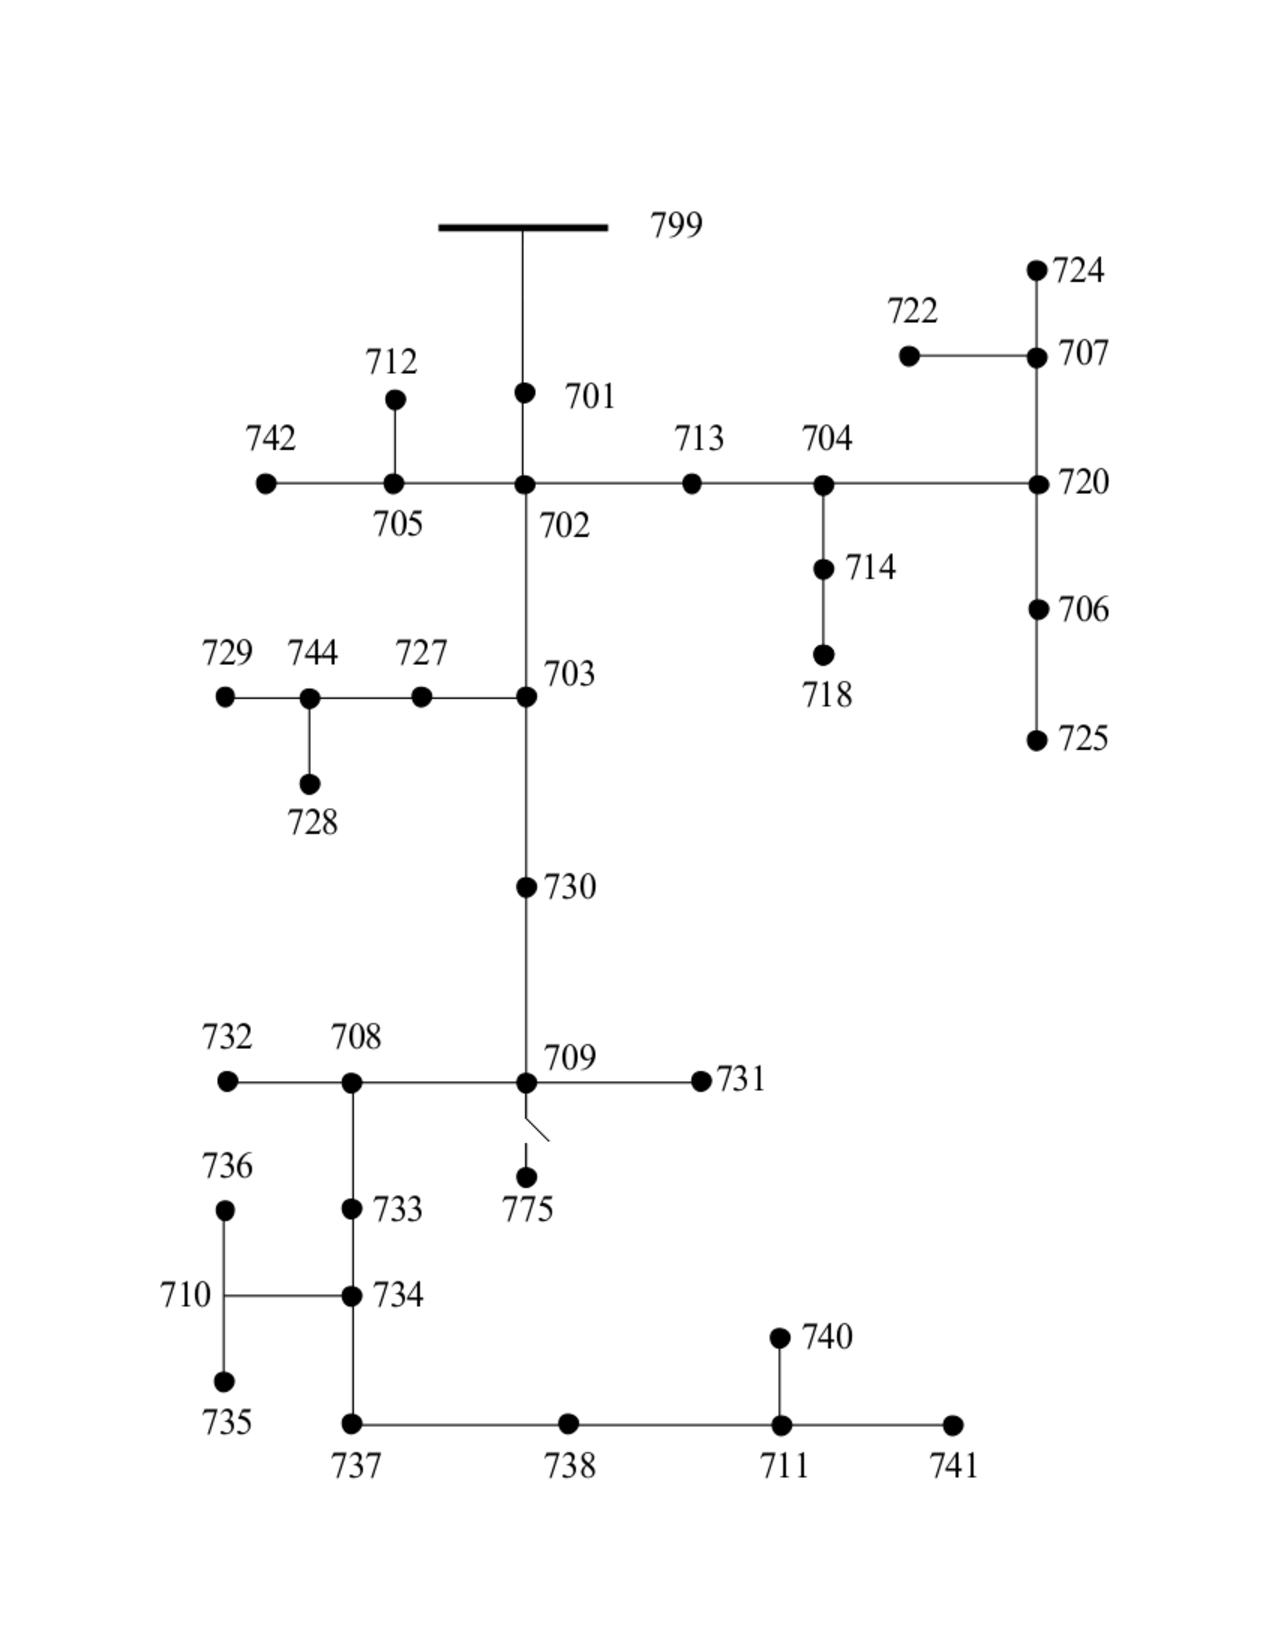
\includegraphics[width=0.375\textwidth, bb={0 0 8500 11000}, trim={2.5cm 2.75cm 2.5cm 3.25cm}, clip]{37nodemod.pdf}
    \caption{Modified IEEE 37 node feeder topology. Note the switch between node 709 and node 775.}
    \label{fig:37nodemod}
\end{figure}
% frame={\fboxrule} {-\fboxrule}

Four-quadrant-capable DER were placed at the following nodes: 702, 704, 725, 724, 729, 732, 735, 737, and 711. We assumed each DER can inject or sink both real and reactive power separately on each phase of the feeder.  The DER were constrained by an apparent power capacity limit on each phase of 300 kVA, or 0.12 pu.

In our experiment, voltage magnitudes were constrained to be within $\pm 5\%$ of 1.0 pu. The voltage at the feeder head was assigned as: 
% $\mathbb{V}_{0} = \begin{bmatrix} 1\angle 0\degree &  1\angle 240\degree & 1\angle 120\degree \end{bmatrix}^{T}$
$\mathbb{V}_{0} = {\left[ 1\angle 0\degree, \text{ } 1\angle 240\degree , \text{ } 1\angle 120\degree \right]}^{T}$
pu. We incorporated the voltage dependent load model of \eqref{eq:sV} with parameters $A_{PQ,n}^{\phi} = 0.9$ and $A_{Z,n}^{\phi} = 0.1 \text{ } \forall \phi \in \{ a,b,c \}, \text{ } \forall n \in \mathcal{N}$.
% We chose the parameters of the \emph{LinDist3Flow} assumptions \textbf{A1} - \textbf{A4} as listed:
% \begin{itemize}
%     \item[]{\textbf{A1}: $\mathbb{L}_{mn} = {\left[ 0, \text{ } 0, \text{ } 0 \right]}^{T} \quad \forall (m,n) \in \mathcal{E}$}
%     \item[]{\textbf{A2}: $\mathbb{H}_{mn} = {\left[ 0, \text{ } 0, \text{ } 0 \right]}^{T} \quad \forall (m,n) \in \mathcal{E}$}
%     \item[]{\textbf{A3}: $\gamma_{n}^{ab} = \sigma$, $ \gamma_{m}^{bc} = \sigma$, $ \gamma_{n}^{ac} = \sigma^{2} \quad \forall n \in \mathcal{N}$}, see Eq. \eqref{eq:sigma}
%     \item[]{\textbf{A4}: $\left| V_{n}^{\phi} \right| = 1 \quad \forall \phi \in \{ a,b,c \}, \text{ } \forall n \in \mathcal{N}$}
% \end{itemize}

In this experiment, we considered switching in an islanded node 775 to the network (i.e. closing the switch between the nodes 709 and 775). To minimize sudden and large real or reactive power flows across the switch and disturbances to the network, we desired to match the voltage phasors at node 709 to that of node 775. To this end, we proposed the following OPF to minimize the voltage phasor difference between one or more nodes and the respective reference at each node, while providing feeder voltage support:
\begin{equation}
\begin{aligned}
  & \underset{u_{n}^{\phi}, v_{n}^{\phi}, y_{n}^{\phi}, \theta_{n}^{\phi}, P_{n}^{\phi}, Q_{n}^{\phi}} {\text{minimize}}
  & & \rho_{y} C_{y} + \rho_{\theta} C_{\theta} + \rho_{w} C_{w} \\
  & \text{subject to}
  & & \eqref{eq:sV}, \eqref{eq:pow_2_lin}, \eqref{eq:mag_7_lin} - \eqref{eq:mag_9_lin}, \eqref{eq:angle_8_lin} \\
  & & & \underline{y} \le y_{n}^{\phi} \le \overline{y} \quad \forall \phi \in \{ a,b,c \}, \text{ } \forall n \in \mathcal{N}, \\
  & & & \left| w_{n}^{\phi} \right| \le \overline{w} \quad \forall \phi \in \{ a,b,c \}, \text{ } \forall n \in \mathcal{N},
\end{aligned}
\label{eq:OPF}
\end{equation}

\noindent where
\begin{align}
C_{y} &= \sum_{n \in \mathcal{N}} \sum_{\phi \in \{a,b,c \}} {\left( y_{n}^{\phi} - y_{ref,n}^{\phi} \right)}^{2}, \label{eq:OPF_Cy} \\
C_{\theta} &= \sum_{n \in \mathcal{N}} \sum_{\phi \in \{a,b,c \}} {\left( \theta_{n}^{\phi} - \theta_{ref,n}^{\phi} \right)}^{2}, \label{eq:OPF_Ctheta} \\
C_{w} &= \sum_{n \in \mathcal{N}} \sum_{\phi \in \{a,b,c \}} {\left| w_{n}^{\phi} \right|}^{2} \label{eq:OPF_Cw}
\end{align}

The OPF objective function is a weighted sum of three terms: $C_{y}$ is the sum of squared magnitude tracking error for all nodes and phases with an assigned magnitude reference, $C_{\theta}$ is the sum of squared angle tracking error for all nodes and phases with an assigned angle reference, and $C_{w}$ is the sum of the squared magnitudes of all DER dispatch.

\setlength{\belowcaptionskip}{0pt}
\setlength{\textfloatsep}{0pt}
\begin{figure}[ht]
	\centering
    \begin{subfigure}{21pc}
        \centering
        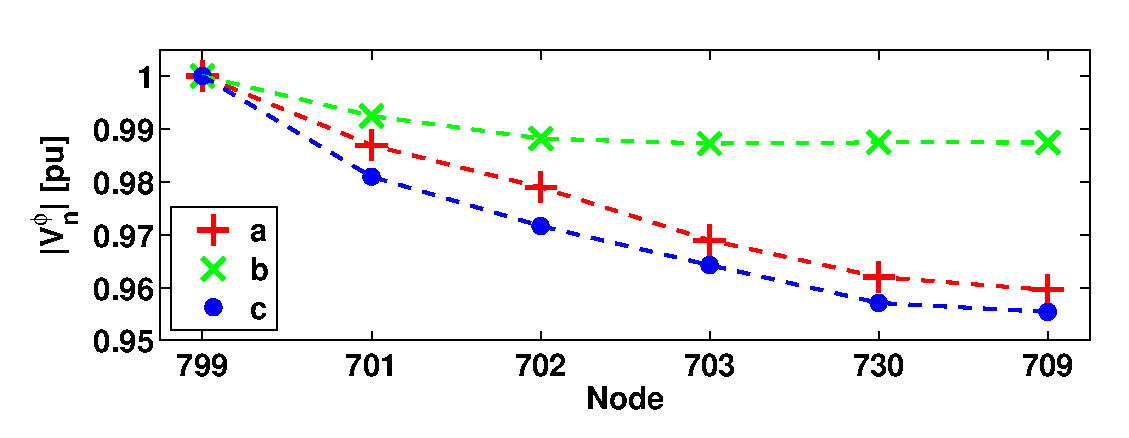
\includegraphics[width=21pc]{track_709path_mag_base}
        \caption{Voltage magnitude profile on path from node 799 to node 709 with no control.}
        \label{fig:track_709path_mag_base}
    \end{subfigure}
    \\
    \begin{subfigure}{21pc}
        \centering
        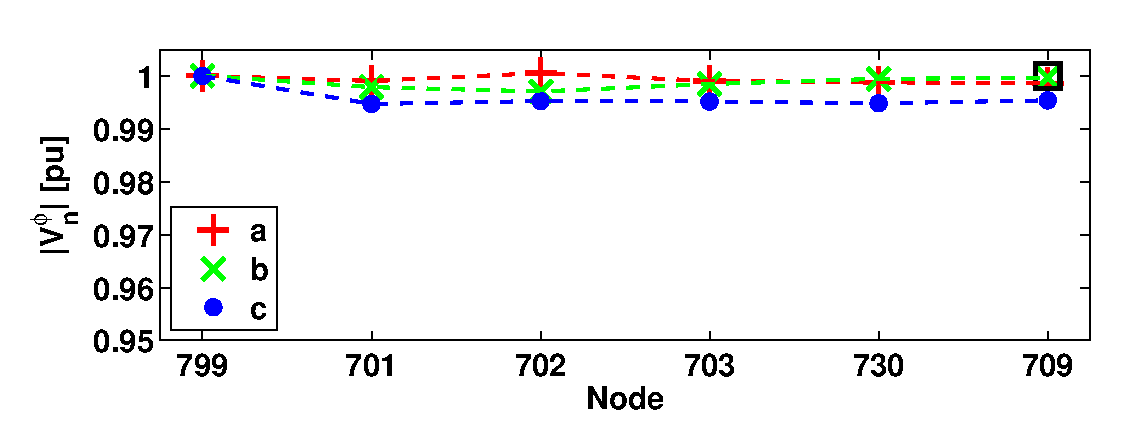
\includegraphics[width=21pc]{track_709path_mag_control}
        \caption{Voltage magnitude profile on path from node 799 to node 709 with control from \eqref{eq:OPF}. The magnitude reference for phases a,b, and c is represented by the black square.}
        \label{fig:track_709path_mag_control}
    \end{subfigure}
    \caption{Comparison of voltage magnitude profiles of base and control cases for phasor reference tracking scenario.}
    \label{fig:track_709path_mag}
    \begin{subfigure}{21pc}
    	\centering
        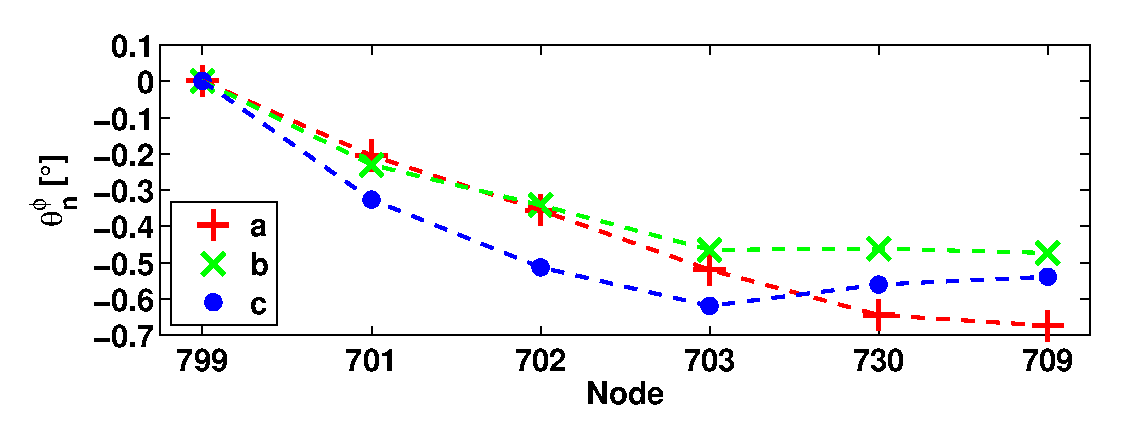
\includegraphics[width=21pc]{track_709path_angle_base}
        \caption{Voltage angle profile on path from node 799 to node 709 with no control.}
        \label{fig:track_709path_angle_base}
    \end{subfigure}
    \\
    \begin{subfigure}{21pc}
        \centering
        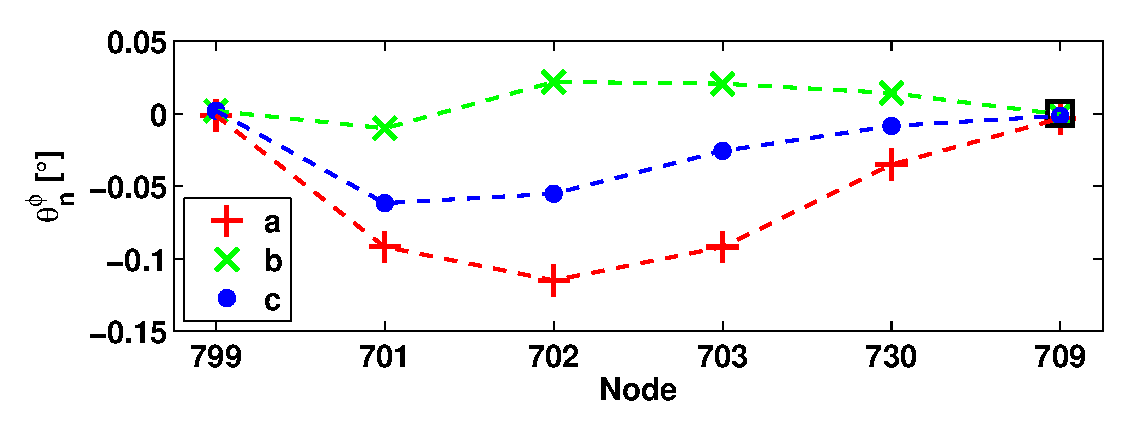
\includegraphics[width=21pc]{track_709path_angle_control}
        \caption{Voltage angle profile on path from node 799 to node 709 with control from \eqref{eq:OPF}. The angle reference for phases $\{ a, b, c \}$ is represented by the black square.}
        \label{fig:track_709path_angle_control}
    \end{subfigure}
    \caption{Comparison of voltage angle profiles for phasor reference tracking scenario. Voltage angles for phases $\{ a, b, c \}$ are referenced to $0\degree$ ($120\degree$ is added to phase b voltage angle and subtracted from phase c voltage angle). The angle reference  is referenced to $0\degree$ in the same manner.}
    \label{fig:track_709path_angle}
\end{figure}

We chose the phasor of node 775 to have unity magnitude ($y_{ref,709}^{\phi} = 1, \text{ } \phi \in \{ a, b, c \}$) and an angle of $0\degree$, $240\degree$, and $120\degree$ for phases a, b and c, respectively ($\theta_{ref,709}^{a} = 0\degree$, $\theta_{ref,709}^{b} = 240\degree$, and $ \theta_{ref,709}^{c} = 120\degree$). Finally, the weights in the objective function were chosen as: $\rho_{y} = 1000, \text{ } \rho_{\theta} = 100, \text{ } \rho_{w} = 1$.

Simulation results, which depict the solution of power flow using the results of \eqref{eq:OPF}, are presented in Figs. \ref{fig:track_709path_mag} - \ref{fig:track_709path_angle}. The voltage magnitude for phases $\{ a, b, c \}$ at nodes along the path from node 799 to node 775 are shown by Fig. \ref{fig:track_709path_mag_base} (a baseline case with no control applied), and Fig. \ref{fig:track_709path_mag_control} (power flow results using the solution of \eqref{eq:OPF} - or the ``control" case). OPF real and reactive power dispatches for controlled nodes can be found in Table \ref{tab:wnode}.  It can clearly be seen that using the dispatch computed by the OPF, the voltage magnitude at node 775 was drastically changed for all three phases and is driven closer to the reference value. Table \ref{table:709voltage} shows the resulting voltage magnitudes at node 709 following the application of control.  Additionally, note that voltage violations in the baseline case have been corrected.  For nodes not depicted in the figures, in the base case simulation all nodes (9 in total) downstream of node 733 had voltage magnitudes lower than 0.95 on phases a and c. These violations were alleviated following the application of control.

The voltage angle on phases $\{ a, b, c \}$ for nodes along the path from node 799 to node 709 is given by Fig. \ref{fig:track_709path_angle_base} for the baseline case, and Fig. \ref{fig:track_709path_angle_control} for the control case, which shows power flow results using the solution of \eqref{eq:OPF}.  As can be seen in the figures, the voltage angles were driven extremely close to the respective references. The resultant voltage angles at node 709 for phases $\{ a, b, c \}$ can be found in Table \ref{table:709voltage}.

\begin{table}[h]
	\centering
    \caption{COMPARISON OF VOLTAGE PHASOR MAGNITUDES AND PHASE ANGLES AT NODE 709.}
	\begin{tabular}{| l | c | c | c |}
		\hline
		Phase & a & b & c \\
		\hline
        Magnitude Reference \hfill [pu] & 1 & 1 & 1 \\
		Base Magnitude \hfill [pu] & 0.9596 & 0.9874 & 0.9554 \\		
		Control Magnitude \hfill [pu] & 0.9987 & 0.9997 & 0.9954 \\
		\hline
        Angle Reference \hfill [$\degree$] & 0 & 240 & 120 \\
		Base Angle \hfill [$\degree$] & -0.6731 & 240.5272 & 119.4613 \\
		Control Angle \hfill [$\degree$] & -0.0034 & 240.9994 & 119.9984 \\
		\hline
    \end{tabular}
    \label{table:709voltage}
\end{table}

% We define the maximum magnitude error for the control case as:
% \begin{equation}
% 	\underset{\phi \in \{ a,b,c \}, \text{ } n \in \mathcal{N}} {\text{maximize}}
% 	\left| V_{n}^{\phi} - V_{n,ref}^{\phi}\right|, \nonumber
% \end{equation}
% \noindent and the maximum angle error for the control case as:
% \begin{equation}
% 	\underset{\phi \in \{ a,b,c \}, \text{ } n \in \mathcal{N}} {\text{maximize}}
% 	\left| \theta_{n}^{\phi} - \theta_{n,ref}^{\phi}\right|. \nonumber
% \end{equation}

\noindent Inspection of Table \ref{table:709voltage} shows, following the application of control, a maximum voltage magnitude error of 0.0046 pu, and a maximum voltage angle error of 0.0034 $\degree$.

\begin{table}[h]
	\centering
    \caption{OPTIMAL DER DISPATCH FROM \eqref{eq:OPF}.}	
    \begin{tabular}{| l | c | c | c |}
    \hline
    & \multicolumn{3}{|c|}{Phase } \\
    \hline
    Node & $a$ $\left( w_{n}^{a} \right)$ [pu] & $b$ $\left( w_{n}^{b} \right)$ [pu] & $c$ $\left( w_{n}^{c} \right)$ [pu] \\
    \hline
    702 & -0.0551 - j0.0587 & -0.0627 - j0.0197 & -0.1079 - j0.0525 \\
    704 & -0.0551 - j0.0588 & -0.0628 - j0.0195 & -0.1079 - j0.0525 \\
    725 & -0.0552 - j0.0588 & -0.0628 - j0.0194 & -0.1079 - j0.0525 \\
    724 & -0.0552 - j0.0588 & -0.0627 - j0.0194 & -0.1079 - j0.0525 \\
    729 & -0.0797 - j0.0833 & -0.0881 - j0.0371 & -0.1078 - j0.0528 \\
    732 & -0.1158 - j0.0314 & -0.0539 - j0.0264 & -0.1095 - j0.0492 \\
    735 & -0.1157 - j0.0318 & -0.0546 - j0.0260 & -0.1095 - j0.0491 \\
    737 & -0.1157 - j0.0318 & -0.0546 - j0.0260 & -0.1095 - j0.0491 \\
    711 & -0.1157 - j0.0320 & -0.0549 - j0.0258 & -0.1095 - j0.0491 \\
    \hline
    \end{tabular}
	\label{tab:wnode}
\end{table}

